% !TeX root = ../../tesi.tex

\subsubsection{Background Subtraction for Motion Triggering}
During the data-acquisition phase, images are not recorded continuously. Instead, the acquisition framework monitors the scene through a configurable background-subtraction stage and stores a frame only when motion is detected inside the selected region of interest (ROI).\cite{opencv_background_subtraction_2026,labby_kinect_acquisition_2026}
\\
In this way, the saved dataset is concentrated around the actual passage of dough balls or bread loaves, while long intervals of static background are discarded.
\begin{figure}[h]
    \centering
    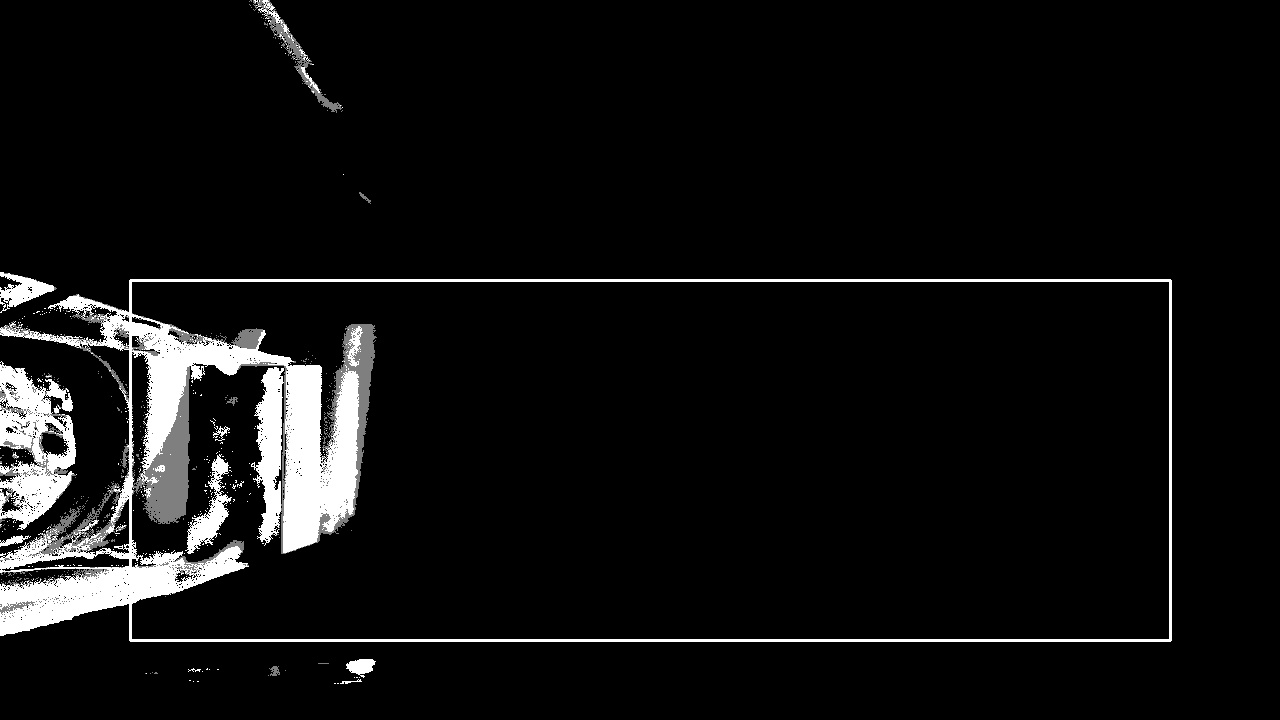
\includegraphics[width=0.8\textwidth]{images/BGS.jpg}
    \caption{Example of background subtraction for motion triggering at Site~2. The operator is placing a tray of bread loaves on the output table. The tray appears as foreground, whereas the table is correctly modelled as background.}
    \label{fig:Background_subtraction2}
\end{figure}

\subsubsection{Implementation details}
The implementation supports the two OpenCV subtractors MOG2 and KNN, both wrapped inside a motion-detection interface that computes a foreground mask and converts it into a normalized motion score.\cite{opencv_background_subtraction_2026,labby_kinect_acquisition_2026} This score is then compared with configurable thresholds in order to decide whether the current frame is relevant enough to be stored. The main parameters of the acquisition logic, such as the selected sensor branch (Kinect\cite{microsoft_azure_nodate} or Raspberry Pi Camera\cite{raspberrypi_camera_module_3_2026}), subtractor type, history length, variance threshold, motion threshold, ROI geometry, image resolution, and initial warm-up offset, are collected in a YAML configuration file (shown in Figure~\ref{fig:YAML_config}) so that the system can be retuned without modifying the source code.\cite{labby_kinect_acquisition_2026}

\begin{figure}[h]
    \centering
    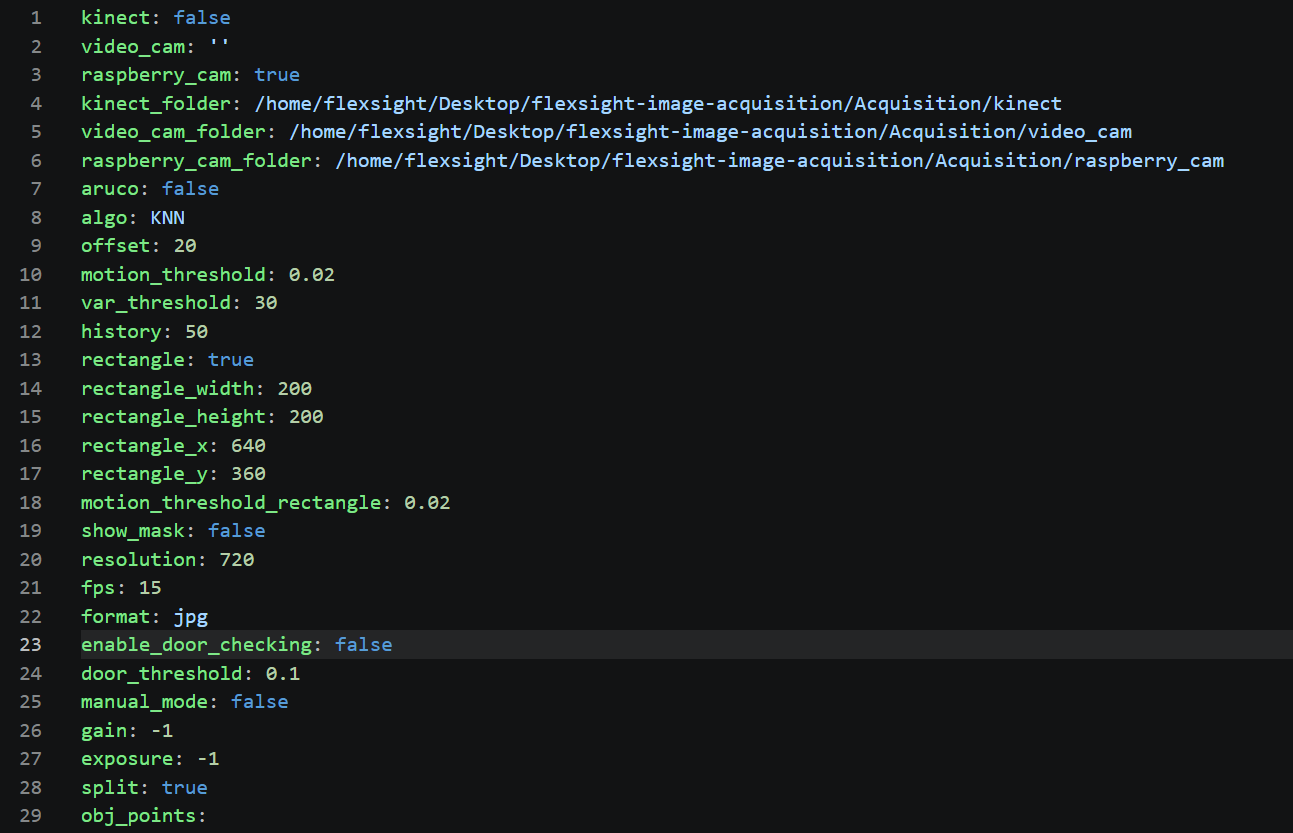
\includegraphics[width=\textwidth]{images/YAML.png}
    \caption{Example of the YAML configuration file used to tune the motion-triggering module without modifying the source code.}
    \label{fig:YAML_config}
\end{figure}

The same logic is reused across the two sites, but the sensing modality depends on the available hardware. In the Kinect branch, ROI-based triggering can be performed on the transformed depth image, the infrared image, or the RGB image. The transformed depth image is particularly convenient because it is substantially invariant to illumination changes. In RGB-only branches, such as the Raspberry Pi acquisition setup used at Site~2, the foreground mask is instead computed directly from the RGB stream.\cite{labby_kinect_acquisition_2026} The framework also skips an initial number of frames in order to stabilize the background model before the actual recording starts, thereby reducing false triggers caused by transient initialization artefacts.

When the motion score exceeds the configured threshold within the selected ROI, the current frame is written to disk together with the modality-specific data associated with the active sensor. In the Kinect setup, the acquisition stage stores RGB, depth, infrared, and mask data. The RGB frames are used for automatic labelling and detector training, whereas the aligned depth data are used to develop and validate the volume-estimation workflow. In the Raspberry Pi setup, the stored outputs are instead the RGB frame and the associated foreground mask, and these data are later used to train the detector and support the downstream bread-analysis pipeline.\cite{labby_kinect_acquisition_2026,labby_thesis_repo_2026} In order to better subdivide the events, the codebase also supports the automatic creation of timestamped folders when motion starts, so that separate acquisition sessions can be organized without manual intervention.\cite{labby_kinect_acquisition_2026}
\newpage
\subsubsection{Data Management and Robustness}
Since the local storage capacity of the embedded devices is limited, the acquisition framework also includes a flushing mechanism that reacts to low-space conditions. When enabled, this mechanism pauses the acquisition logic and allows the oldest files to be transferred to an external SSD, thereby freeing local space for new data.\cite{labby_kinect_acquisition_2026} This feature is particularly useful during long autonomous campaigns, where the amount of generated data can quickly exceed the internal storage capacity of the device.

\begin{figure}[h]
    \centering
    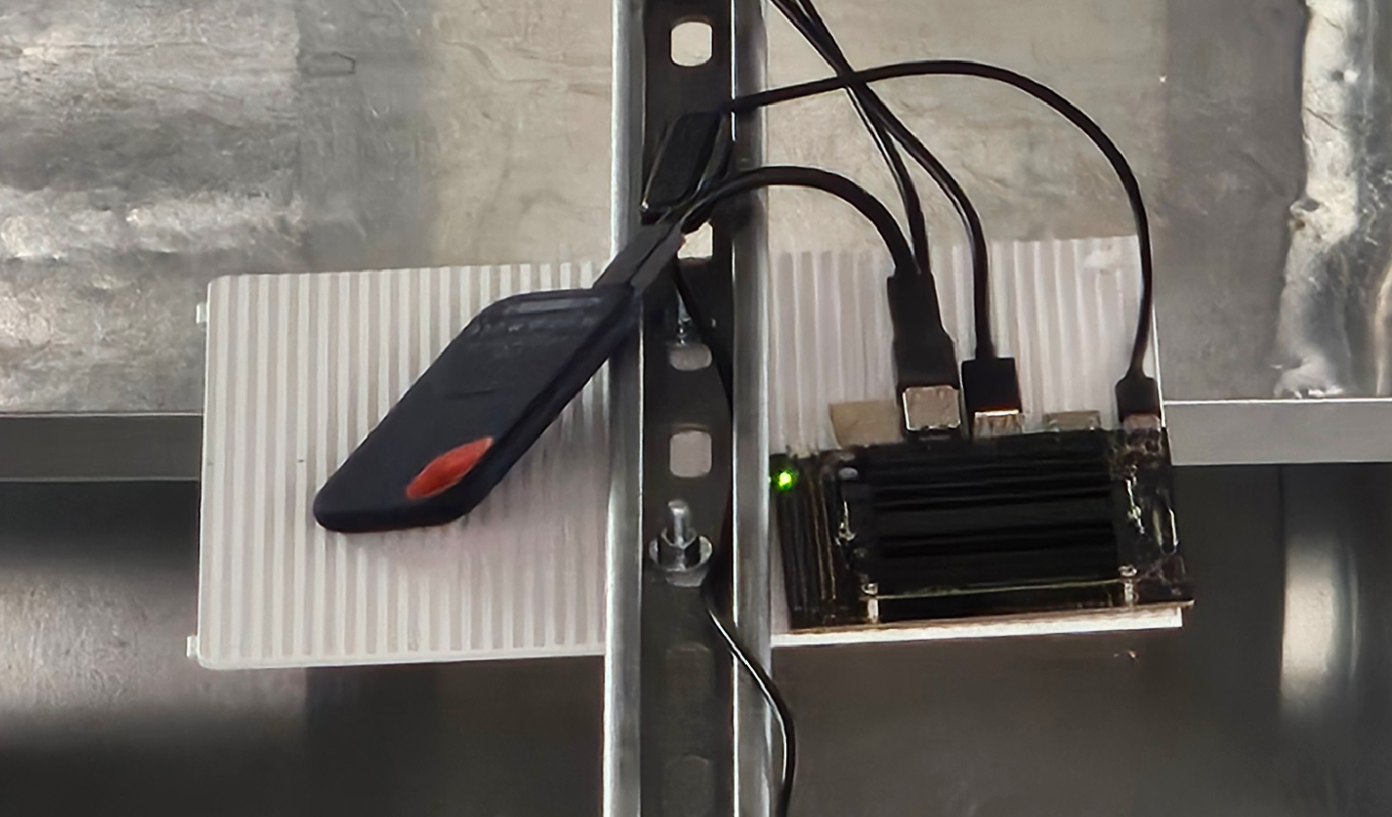
\includegraphics[width=0.5\textwidth]{images/ssd.PNG}
    \caption{Jetson Nano with the external SSD used for data flushing during long acquisition campaigns.}
    \label{fig:SSD_flushing}
\end{figure}

To further increase robustness, the acquisition scripts can be launched automatically at startup through system services or desktop autostart entries, so that the data-collection process can resume after power interruptions or device reboots without requiring manual intervention.\cite{labby_kinect_acquisition_2026,systemd_service_2026} As discussed in Chapter~1, this aspect was essential for ensuring continuity during two-week acquisition campaigns in an industrial environment.

Overall, this motion-triggered acquisition strategy proved particularly suitable for long autonomous campaigns, because it reduces redundant storage while preserving the samples that are most informative for the subsequent labelling and training stages. At the same time, the framework remains modular enough to support different sensors and acquisition modes without requiring a complete redesign of the system.\cite{labby_kinect_acquisition_2026}
